\begin{figure}[h]
\centering
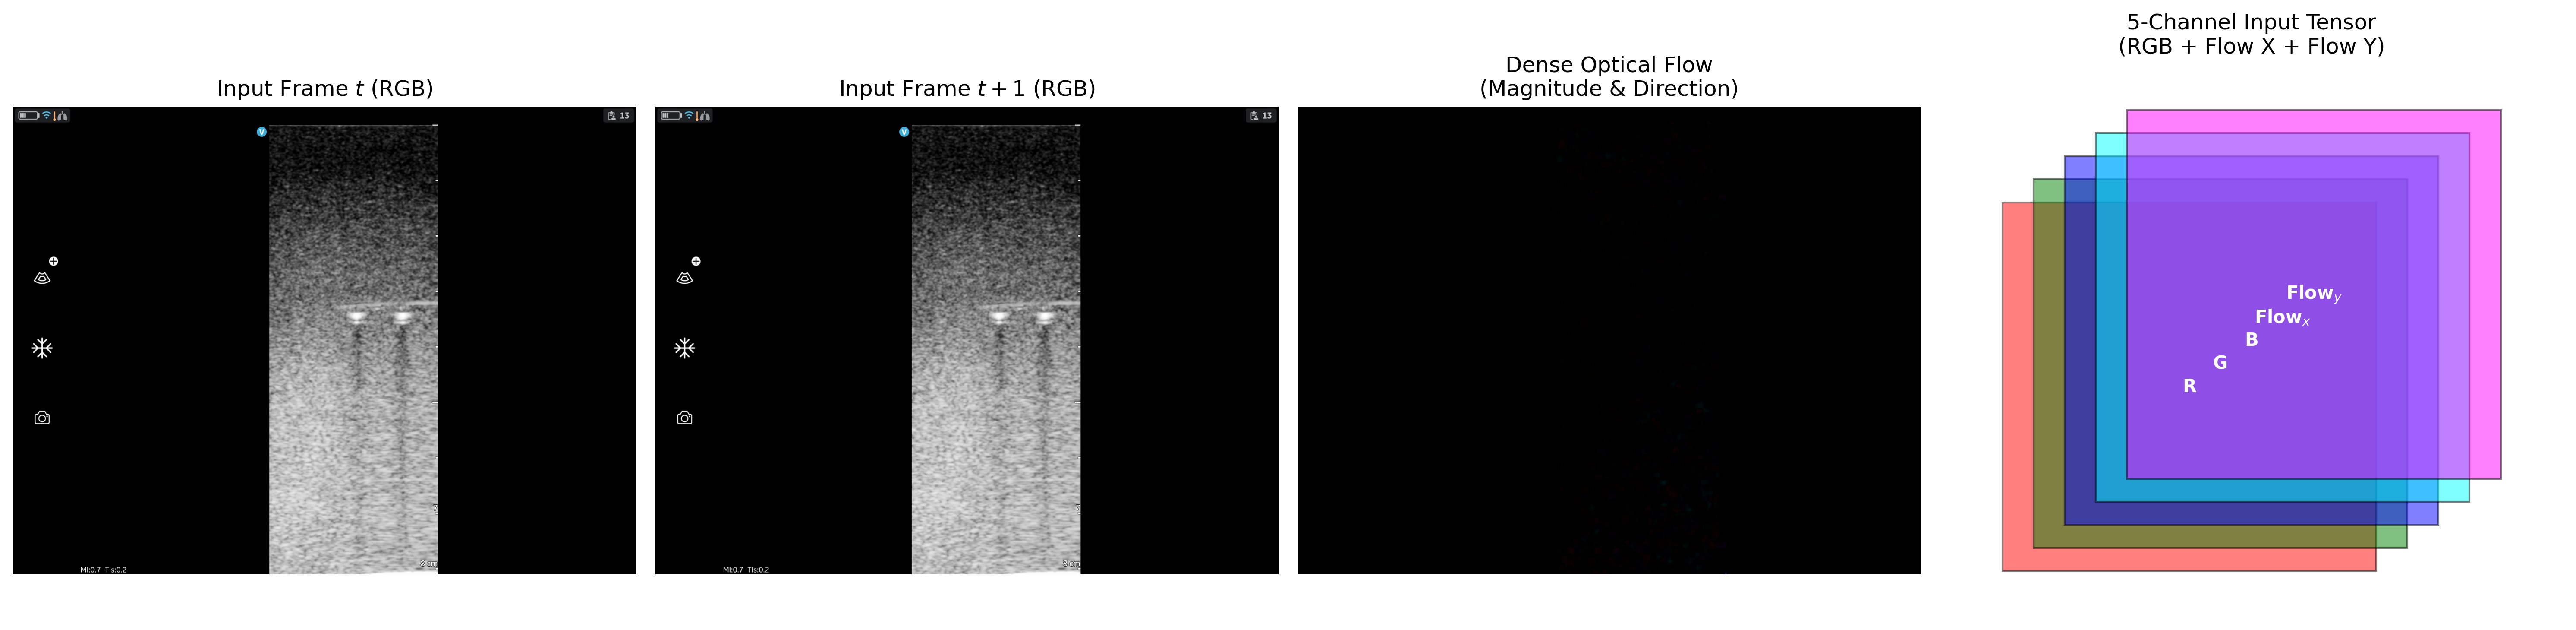
\includegraphics[width=1.0\textwidth]{paper/figures/preprocessing_pipeline.png}
\caption{Data Preprocessing Pipeline. Ultrasonic video frames are processed to extract (1) RGB channels normalized via ImageNet statistics, and (2) dense optical flow fields (Farneback algorithm) capturing motion-induced temperature cues. The 5-channel input representation explicitly encodes both appearance and temporal dynamics, enabling the network to detect subtle convective heat patterns and flow artifacts.}
\label{fig:preprocessing_pipeline}
\end{figure}
